\chapter{Trace Encoder Output Packets} \label{packets}

Figure~\ref{fig:packet-format} gives an example of a possible basic structure for 
packets emerging from the encoder, in network order (1st transmitted byte is on the left).
This shows how the payload maybe encapsulated.  The header includes the packet length, and 
the index identifies the source of the packet.  
Different instantiations or implementations may have different encapsulating structures.  
This will typically be dependent upon such things as the trace routing infrastructure within the 
SoC.  In order to support this, the encoder must provide the following information to the encapsulator:

\begin{itemize}
  \item The packet type;
  \item The packet length, in bytes;
  \item The packet payload.
\end{itemize}

The remainder of this section describes the contents of the Payload
portion which should be independent of the infrastructure.  In each table, the fields are listed in
transmission order: first field in the table is transmited first, and multi-bit fields are 
transmitted LSB first.

\begin{figure}[h]
\begin{center}
  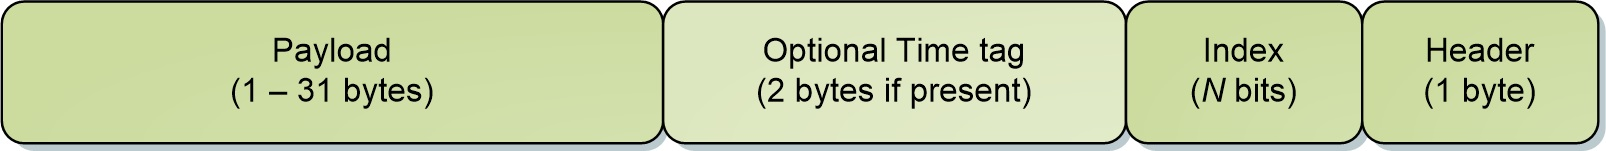
\includegraphics[height=1cm, width=9cm]{newPacket.jpg}
  \caption{Example Encapsulated Packet Format}
  \label{fig:packet-format}
\end{center}
\end{figure}


This packet payload format is used to output encoded instruction
trace.  Four different formats are used according to the needs of the
encoding algorithm. The following tables show the format of the
payload - i.e. excluding any encapsulation.

In order to achieve best performance, actual packet lengths may be adjusted using 'sign based compression'.
At the very minimum this should be applied to the address field, but ideally will be applied to the whole 
packet.  This technique eliminates identical bits from the most significant end of the packet, and adjusts
the length of the packet accordingly.  A decoder receiving this shortened packet can reconstruct the 
original full-length packet by sign-extending from the most significant received bit.  An example of how
this technique is used to choose between address formats is given in Section~\ref{addresses}.  The same
principal can be applied to the entire packet, and the length (typically given in bytes) adjusted 
accordingly.

Where the payload length given in the following tables, or after applying sign-based compression, is not a 
multiple of whole bytes in length, the payload must be sign-extended to the nearest byte boundary.

\begin{table}[htp]
    \centering
    \caption{Packet Payload Format 0 and 1}
    \label{tab:te_inst0-1}
    \begin{tabulary}{\textwidth}{|l|p{35mm}|p{80mm}|}
        \hline
        {\bf Field name} & {\bf Bits} & {\bf Description} \\
        \hline
        \textbf{format}	& 2	& 00 (full-delta): includes branch map and full address \newline
                        01 (diff-delta): includes branch map and differential address\\
        \hline
        \textbf{branches} & 5 & Number of valid bits in branch-map. The length of branch-map is determined as follows: \newline
        0:      31 bits (\textbf{address} is not valid) \newline
        1: 	1 bit \newline
        2-9: 	9 bits \newline
        10-17: 	17 bits \newline
        18-25: 	25 bits \newline
        26-31: 	31 bits \newline
        For example if branches = 12, the branch-map is 17 bits long, and the 12 LSBs are valid. \newline
        In most cases when the branch map is full there is no need to report an address,
        and this is indicated by setting branches to 0.  The exception to this is when 
        the instruction immediately prior to the final branch causes an unpredictable discontinuity.\\
        \hline
        \textbf{branch-map} & Number of bits \newline 
                     determined by \newline 
                     \textbf {branches} field & 
                     An array of bits indicating whether branches are taken or not.\newline
        Bit 0 represents the oldest branch instruction executed.   For each bit: \newline
        0: branch taken \newline
        1: branch not taken \\
        \hline
        \textbf{address}	& Number of bits \newline 
                  is \textit {iaddress\_width\_p - iaddress\_lsb\_p} & 
                    Differential or full instruction address, according to \textbf {format}.  \newline
                    When branches is 0, the address is invalid, and is formed by sign extending branch-map.\\
        \hline
    \end{tabulary}
\end{table}


\begin{table}[!h]
    \centering
    \caption{Packet Payload Format 2}
    \label{tab:te_inst2}
    \begin{tabulary}{\textwidth}{|l|p{35mm}|p{80mm}|}
        \hline
        {\bf Field name} & {\bf Bits} & {\bf Description} \\
        \hline
        \textbf{format}	& 2	& 10 (addr-only): address and no branch map\\
        \hline
        \textbf{address} & Total number of bits 
                  for address is
                  \textit {iaddress\_width\_p - iaddress\_lsb\_p}. & 
                  Address is always differential unless the encoder has been configured to only use full-address\\ 
        \hline
    \end{tabulary}
\end{table}

\begin{table}[htp]
    \centering
    \caption{Packet Payload Format 3}
    \label{tab:te_inst3}
    \begin{tabulary}{\textwidth}{|l|p{35mm}|p{80mm}|}
      \hline
          {\bf Field name} & {\bf Bits} & {\bf Description} \\
          \hline
          \textbf{format} & 2 & 11 (sync): synchronisation\\
          \hline
          \textbf{subformat} & 2 & Sync sub-format omits fields when not required: \newline
          00 (start): ecause, interrupt and tval omitted \newline
          01 (exception): All fields present\newline
          10 (context): \textbf{address, branch, ecause, interrupt} and \textbf {tval} omitted \newline
          11 : reserved \\
          \hline
          \textbf{context} &  Total number of bits 
                     for context is  
                     \textit {context\_width\_p} 
                     unless  
                     \textit {nocontext\_p} is 1,  
                     in which case it is 0 & 
                     The instruction context \\
          \hline
          \textbf{privilege} & Number of bits is  
                      \textit {privilege\_width\_p} & 
                      The current privilege level \\
          \hline
          \textbf{branch} & 1 & If the address points to a branch instruction, set to 1 if the branch was not taken. 
          Has no meaning if this instruction is not a branch. \\
          \hline
          \textbf{address} & number of bits is  
                    \textit {iaddress\_width\_p - iaddress\_lsb\_p},  
                    unless subformat is 10, & 
                    Full instruction address.  Address alignment is determined by \textit {iaddress\_lsb\_p} Address must be left shifted in order to recreate original byte address \\
          \hline
          \textbf{ecause} & Number of bits is  
                   \textit {ecause\_width\_p} if  
                   subformat is 01,  
                   or 0 otherwise  
                   (no exception). & 
                   Exception cause \\
          \hline
          \textbf{interrupt} & Number of bits is  
                      1 if subformat is 01,  
                      or 0 otherwise (no exception). & 
                      Interrupt \\
          \hline
          \textbf{tval} & Number of bits is  
                 \textit {iaddress\_width\_p}  
                 if subformat is  
                 01 and \textit {notval\_p} is 
                 0, or 0 otherwise  
                 (no exception). & 
                 Trap value \\
          \hline
    \end{tabulary}
\end{table}

\begin{table}[!h]
    \centering
    \caption{te\_support payload}
    \label{tab:te_support}
    \begin{tabulary}{\textwidth}{|l|p{8mm}|p{80mm}|}
        \hline
        \textbf {Field name} & \textbf {Bits} & \textbf {Description} \\
        \hline
        \textbf{support\_type} & 4 & Set to 0 to indicate instruction trace status \\
        \hline
        \textbf{enable} & 1 & Indicates if encoder is enabled\\
        \hline
        \textbf{encoder\_mode} & N & Identifies trace algorithm\newline
          Details implementation dependent.  Currently Branch trace is the only mode defined.\\
        \hline
        \textbf{qual\_status} & 2 & Indicates qualification status\newline
          00 (no\_change): No change to filter qualification \newline
          01 (ended\_rep): Qualification ended, preceding \textbf{te\_inst} sent explicitly to indicate last qualification instruction\newline
          10: Reserved\newline
          11 : (ended\_ntr): Qualification ended, no unreported instructions (so preceeding \textbf{te\_inst} would have been sent anyway, even if it wasn't the last qualified instruction)\\
        \hline
        \textbf{options} & N & Values of all run-time configuration bits\newline
          Number of bits and definitions implementation dependent.  Examples might be\newline
          - Always output full addresses (SW debug option)\newline
          - Exclude address from format 3, sub-format 1 \textit{te\_inst} packets if trap vector can be determined from \textit{ecause field}\newline
          - Don't report function return addresses\\
          \hline
    \end{tabulary}
\end{table}

\begin{table}[!h]
    \centering
    \caption{packet\_lost payload}
    \label{tab:te_support}
    \begin{tabulary}{\textwidth}{|l|p{8mm}|p{80mm}|}
        \hline
        \textbf {Field name} & \textbf {Bits} & \textbf {Description} \\
        \hline
        \textbf{high\_loss} & 1 & Qualitative indication of loss severity.  Heuristic is implementation specific.\\
        \hline
        \textbf{lost\_stream} & N & Identifies the source of lost packets\newline
          Number of bits and encoding implementation specific.  Provides for encoders to independently indicate loss of 
          different types of packets (e.g. instruction trace, data trace, etc.)\\
        \hline
    \end{tabulary}
\end{table}
